% Paper C — NeurIPS 2026 (P2 in NEURIPS_SUBMISSIONS.md)
% Locked title and abstract from paper/abstracts/ABSTRACT_NEURIPS_v3 (P1
% lineage) and paper/drafts/NEURIPS_SUBMISSIONS.md §P2 (this paper).
% Spine: three ideologies of recurrent memory in pretrained LLMs;
% organising principle for the six failure modes and the audit battery.
\documentclass{article}

\usepackage[preprint]{neurips_2024}
\usepackage[utf8]{inputenc}
\usepackage[T1]{fontenc}
\usepackage{hyperref}
\usepackage{url}
\usepackage{booktabs}
\usepackage{amsfonts}
\usepackage{amsmath}
\usepackage{amssymb}
\usepackage{microtype}
\usepackage{xcolor}
\usepackage{graphicx}
\usepackage{multirow}
\usepackage{makecell}
\setcitestyle{numbers,square}

\newcommand{\Mc}{M_{\mathrm{c}}}
\newcommand{\Ct}{C_t}
\newcommand{\mt}{m_t}
\newcommand{\Min}{M_{\mathrm{in}}}
\newcommand{\Mj}{M_{\mathrm{judge}}}
\newcommand{\Mnew}{M_{\mathrm{new}}}
\newcommand{\dnm}{\Delta_{\mathrm{nm-m}}}
\newcommand{\dsh}{\Delta_{\mathrm{sh-m}}}
\newcommand{\CEmem}{\mathrm{CE}_{\mathrm{mem}}}
\newcommand{\CEnomem}{\mathrm{CE}_{\mathrm{nomem}}}
\newcommand{\CEsh}{\mathrm{CE}_{\mathrm{shuffle}}}
\newcommand{\CEfloor}{\mathrm{CE}_{\mathrm{floor}}}
\newcommand{\elift}{\Delta_{\mathrm{evidence}}}
\newcommand{\amem}{\alpha_{\mathrm{mem}}}

\title{When Does Recurrent Memory Help?\\
       Six Failure Modes and a Methodology for Honest Evaluation of Augmented LLMs}

\author{%
  Anonymous Authors\\
  \texttt{anonymous@example.com}
}

\begin{document}

\maketitle

\begin{abstract}
We began with a simple question: why did a recurrent memory module
sometimes look useful, sometimes invisible, and sometimes actively
harmful on the same long-conversation callback task?  In a
$16$-version campaign on Memory Residuals --- a slot-attention memory
matrix attached to Qwen3-0.6B and Qwen3-1.7B --- the answer was not a
single bug.  It was an evaluation problem.  Token-averaged chain
evaluation diluted a localized callback gain by roughly two orders of
magnitude; frozen and joint training measured different causal
pathways; the synthetic D4v2 callback template leaked a $32$-way
category prior that joint-trained models matched directly; more than
half of the D4v2 callback windows exposed evidence to the LM path;
evidence redaction had to be audited before a zero lift could be
trusted; and a random-ID corpus removed the prior but exposed a
writer objective that still did not force chain-specific bindings into
$\Mc$.  We turn these failures into a six-item methodology:
callback-aware evaluation, evidence-redacted memory floors, empirical
and base-model prior audits, window-leakage counts, a test-time
readout audit that asks whether the writer encoded the answer at all,
and a held-out-corpus pivot that breaks the templated-data confound.
Applying the methodology end-to-end yields a single positive recipe
--- a frozen pretrained backbone with a fixed-size jointly-trained
$\Mc$, supervised by LM-NLL alone --- that delivers
$+1.32 \pm 0.53$~nats of chain-specific callback CE improvement on
LongMemEval-S validation across four seeds at Qwen3-0.6B, with a
chain-shuffle confound statistically zero.  The methodology rejects
all of our earlier published-looking results.
\end{abstract}

\section{Introduction}
\label{sec:intro}

A practical conversational agent should remember a user across
sessions.  Three architectural routes for that capability dominate
the contemporary literature: \emph{joint training}, in which a memory
module and the language-model backbone are trained together
end-to-end; \emph{frozen backbone}, in which a small recurrent state
is added to a pretrained model whose parameters are then held fixed;
and \emph{retrieval}, in which past sessions are indexed and re-fed
through the attention window at query time.  Papers in each of the
three programs report success.  Papers from the three programs
rarely fail in the same way.  And papers from the three programs
rarely report the same evaluation controls.

This paper contains a finding that does not look like a finding when
described in any one of the three vocabularies.  In a $16$-version
post-mortem of \emph{Memory Residuals} --- a slot-attention recurrent
memory module attached to Qwen3-0.6B and Qwen3-1.7B that we are able
to train under all three regimes on the same architecture --- we
encountered six independent failure modes.  Each is sufficient by
itself to make a published-style result look positive when the result
is not actually carrying chain-specific information.  Five of the six
have been observed individually, in one or another of the three
research programs, but never together; the sixth (writer-objective
failure) is, to our knowledge, novel as a documented memory-side
pathology.  The failure modes are independent: fixing one does not
fix the others.

The diagnostic state of the literature is that each program checks
roughly the failure modes the others do not.  A joint-training paper
typically reports task accuracy and a no-memory baseline, which dodges
token-averaging dilution but leaves the joint-training-invisibility
mode and the template-prior leak unmeasured.  A frozen-backbone paper
typically reports a chain-CE delta, which exposes the
joint-invisibility mode by construction but masks token-averaging
dilution and rarely reports an evidence-redacted floor.  A retrieval
paper typically reports a recall@$k$ and a downstream-QA accuracy,
which catches some surface-form leakage but does not address the
chain-shuffle confound.  Cross-program, no single paper to our
knowledge reports all six controls; most report two or fewer (Table
\ref{tab:ideologies}).

\paragraph{Contributions.}  This paper makes three contributions and
one empirical surprise.

\begin{enumerate}\setlength{\itemsep}{0.5pt}
\item \textbf{A field-level diagnosis.}  Three research programs of
recurrent memory (joint training, frozen backbone, retrieval) cluster
into three evaluation conventions whose reporting matrices do not
overlap.  We describe and tabulate the gap (\S\ref{sec:ideologies}).
\item \textbf{Six failure modes (\S\ref{sec:failure_modes}).}  We
catalogue six independent ways a recurrent-memory result can look
positive without carrying chain-specific information; each is
load-bearing on at least one ideology, each is detected by a single
cheap diagnostic, and we exhibit a worked numerical example from the
campaign for each.
\item \textbf{Six-item audit methodology (\S\ref{sec:methodology}).}
Callback-aware evaluation, evidence-redacted memory floors, empirical
and base-model prior audits, window-leakage counts, a test-time
readout audit, and a held-out-corpus pivot.  Total compute cost
$<\!1$~H100-hour per checkpoint, applies to all three ideologies.
\item \textbf{An empirical surprise (\S\ref{sec:f3_off}).}  The
auxiliary readout-probe loss that the joint-training literature
canonically prescribes for the writer-objective failure mode is, in
our setting, \emph{harmful}: removing it multiplies $\dnm$ by
$\sim\!8\times$ at both 0.6B and 1.7B, with a chain-level paired
permutation test giving $p < 10^{-4}$.  The recipe that survives all
six audits is the simpler, probe-free one
(\S\ref{sec:recipe_survived}).
\end{enumerate}

The negative claims are bracketed where they have to be: we describe
in \S\ref{sec:claims} which of the six failure modes generalize by
construction (those that live in the metric or the corpus, not the
architecture), and which we observe only in our specific
slot-attention recipe at $\le 1.7$B.

\section{Three Ideologies of Recurrent Memory in Pretrained LLMs}
\label{sec:ideologies}

We use the word \emph{ideology} in the modest sense of a research
program with its own characteristic evaluation conventions; nothing
in this paper rests on a stronger philosophical reading.  The three
programs are not interchangeable engineering choices.  Each makes a
different bet about where the chain-specific binding lives, each is
exposed to a different subset of the failure modes catalogued in
\S\ref{sec:failure_modes}, and each tends to report a different
subset of controls.

\paragraph{Joint training.}  The bet is that gradient descent over
the entire model will allocate credit to whichever path carries the
chain-specific binding.  Examples: AutoCompressors~\cite{autocompressors2023},
Memorising Transformers~\cite{memorizing2022}, TRIME~\cite{trime2022},
RIMs~\cite{rmt2022}, the differentiable-memory family
(NTM~\cite{ntm2014}).  This program is exposed by construction to
\emph{joint-training invisibility} (FM2, \S\ref{sec:fm2}) and to
\emph{template-prior leak} (FM3, \S\ref{sec:fm3}): when there is more
than one path through which the LM head can solve the callback,
gradient descent allocates credit to the easier one, and the memory
channel can collapse to noise.

\paragraph{Frozen backbone.}  The bet is that freezing the LM head
removes the non-memory paths by construction; if memory helps,
the help has to come through $\Mc$.  Examples: the Recurrent Memory
Transformer in its frozen-LM ablation~\cite{rmt2022,armt2024},
Block-Recurrent Transformer~\cite{blockrecurrent2022}, the Compressive
Transformer~\cite{compressive2019}.  The Memory Residuals primitive
we use as a substrate falls in this program.  This program escapes
FM2/FM3 but is heavily exposed to \emph{token-averaged dilution} (FM1,
\S\ref{sec:fm1}) --- a frozen backbone's CE delta is small relative
to the score window --- and to \emph{redaction uncertainty} (FM5,
\S\ref{sec:fm5}): a zero evidence-lift could mean either a
content-blind writer or a leaky redaction.  Without an audit, the two
cannot be distinguished.

\paragraph{Retrieval.}  The bet is that recurrent state is
unnecessary: index past sessions, retrieve at query time, append to
context.  Examples: RAG~\cite{ragoriginal2020}, the kNN variant of
Memorising Transformers~\cite{memorizing2022}, DOS-RAG~\cite{ragbaseline2025}.
This program is exposed to \emph{window leakage} (FM4,
\S\ref{sec:fm4}) by construction, since retrieved evidence enters the
LM attention window deliberately, and to surface-form/literal-match
shortcuts that the long-context-evaluation literature
\cite{nolima2025,ruler2024,lostmiddle2024} has documented for
retrieval but rarely connected back to memory architectures.

\begin{table}[t]
\centering
\caption{Reporting matrix.  Of the six diagnostics catalogued in
\S\ref{sec:failure_modes}, which are reported in representative
papers from each ideology and from the long-context-evaluation
cluster.  $\checkmark$ = reported with quantitative evidence;
$\sim$ = partially addressed (mentioned, implicitly controlled, or
addressed for a related concern); $-$ = not reported.  Columns:
``CB-CE'' callback-aware CE (vs aggregate); ``Floor''
evidence-redacted memory floor; ``Prior'' empirical or base-model
prior baseline; ``WLk'' window-leakage count; ``Red.'' redaction
validity audit; ``TTT'' test-time readout audit.  Cell judgments
follow the per-paper notes in our literature audit
(Appendix~\ref{app:litaudit}); partial credit is given where a
paper's stated controls plausibly cover a diagnostic even if it is
not named the same way.  No paper in the audit reports more than
two of the six diagnostics with quantitative evidence.}
\label{tab:ideologies}
\small
\begin{tabular}{llcccccc}
\toprule
Paper & Ideology & CB-CE & Floor & Prior & WLk & Red. & TTT \\
\midrule
Memorising Transformers~\cite{memorizing2022}     & joint     & $-$    & $-$    & $-$           & $-$           & $-$ & $-$    \\
AutoCompressors~\cite{autocompressors2023}        & joint     & $-$    & $\sim$ & $-$           & $-$           & $-$ & $-$    \\
TRIME~\cite{trime2022}                             & joint     & $-$    & $-$    & $\sim$        & $-$           & $-$ & $-$    \\
RIMs~\cite{rims2021}                               & joint     & $-$    & $-$    & $-$           & $-$           & $-$ & $-$    \\
NTM/DNC~\cite{ntm2014}                             & joint     & $-$    & $-$    & $-$           & $-$           & $-$ & $-$    \\
RMT-frozen~\cite{rmt2022}                          & frozen    & $-$    & $-$    & $-$           & $-$           & $-$ & $-$    \\
ARMT~\cite{armt2024}                               & frozen    & $-$    & $-$    & $-$           & $-$           & $-$ & $-$    \\
Block-Recurrent~\cite{blockrecurrent2022}         & frozen    & $-$    & $-$    & $-$           & $-$           & $-$ & $-$    \\
Compressive Tr.~\cite{compressive2019}             & frozen    & $-$    & $-$    & $-$           & $-$           & $-$ & $-$    \\
RAG~\cite{ragoriginal2020}                         & retrieval & $-$    & $-$    & $-$           & $\sim$        & $-$ & $-$    \\
DOS-RAG~\cite{ragbaseline2025}                     & retrieval & $-$    & $-$    & $\sim$        & $\sim$        & $-$ & $-$    \\
NoLiMa~\cite{nolima2025}                           & long-ctx  & $-$    & $-$    & $\checkmark$  & $\checkmark$  & $-$ & $-$    \\
RULER~\cite{ruler2024}                             & long-ctx  & $-$    & $-$    & $\checkmark$  & $\checkmark$  & $-$ & $-$    \\
Lost-in-the-Middle~\cite{lostmiddle2024}           & long-ctx  & $-$    & $-$    & $\sim$        & $-$           & $-$ & $-$    \\
LongBench~\cite{longbench2024}                     & long-ctx  & $\sim$ & $-$    & $\checkmark$  & $-$           & $-$ & $-$    \\
BABILong~\cite{babilong2024}                       & long-ctx  & $-$    & $-$    & $\sim$        & $\sim$        & $-$ & $-$    \\
ZeroSCROLLS~\cite{zeroscrolls2023}                 & long-ctx  & $-$    & $-$    & $\sim$        & $-$           & $-$ & $-$    \\
LongMemEval~\cite{longmemeval2025}                 & long-ctx  & $\sim$ & $-$    & $\sim$        & $\sim$        & $-$ & $\sim$ \\
\textbf{This paper}                                & all three & $\checkmark$ & $\checkmark$ & $\checkmark$ & $\checkmark$ & $\checkmark$ & $\checkmark$ \\
\bottomrule
\end{tabular}
\end{table}

The pattern in Table \ref{tab:ideologies} is the field-level
finding.  No paper in our audit reports more than two of the six
diagnostics with quantitative evidence, and the diagnostics that do
appear are concentrated in the long-context-evaluation cluster
(NoLiMa, RULER, LongBench) where they have been imported as a
\emph{retrieval} or \emph{benchmark-design} concern but not yet
re-exported back into \emph{memory-architecture} evaluation.

\paragraph{Why this matters.}  An honest evaluation of recurrent
memory has to rule out the failure modes its own ideology is blind to
and the failure modes the other two ideologies are sensitive to.
None of the three programs is self-validating.  The contribution of
this paper is to consolidate the controls into a single battery
that survives across all three.

\section{Memory Residuals as a Cross-Regime Substrate}
\label{sec:memres}

We use Memory Residuals as a substrate, not as a proposed method.
It is, to our knowledge, the only recurrent-memory architecture
that admits all three ideological framings on the same parameter
count and same corpus, which is what makes the cross-regime
comparison in this paper possible.  Briefly: a fixed-size memory
matrix $\Mc \in \mathbb{R}^{K \times d}$ with $K=128$ slots is
updated at session boundaries via a two-stage Extract+Judge
slot-attention writer, and read back into the LM through a
depth-routed cross-attention residual; we denote the readout's
contribution to the residual stream by $\mt$.  A learned routing
mass $\amem$ controls the share of the LM computation that uses
the memory source at each routed sublayer.  Architecture and
training-recipe details are deferred to Appendix \ref{app:arch}.

The same code path supports three regimes by changing only the
\texttt{--freeze\_backbone}, \texttt{--readout\_probe\_loss\_weight},
and \texttt{--retrieval\_index} CLI flags: \emph{joint training}
(unfrozen backbone, no auxiliary), \emph{frozen backbone} (frozen
backbone, $\Mc$-only training), and \emph{retrieval-paired} (frozen
backbone, $\Mc$ replaced by retrieved-context concatenation).  All
six failure modes catalogued in the next section are exhibited on
this single architecture under the appropriate regime.

\section{Six Failure Modes}
\label{sec:failure_modes}

\begin{figure}[t]
\centering
\fbox{\begin{minipage}{0.94\linewidth}
\small
\textbf{Five pathways from $\Mc$ or context to the LM head.}  Only
the first is chain-specific recurrent memory; the other four are
the failure modes we catalogue.
\begin{enumerate}\setlength{\itemsep}{0pt}
\item \emph{Intended path} (chain-specific memory):
  evidence session $\rightarrow \Ct \rightarrow$ writer
  $\rightarrow \Mc \rightarrow \mt \rightarrow$ LM head.
\item \emph{Content-blind memory prior} (FM6, the writer-objective
  failure): writer emits a similar $\Mc$ on every chain; the readout
  shifts the LM toward the callback marginal regardless of evidence.
\item \emph{Backbone template prior} (FM2, FM3): unfrozen LM learns
  $P(\text{item} \mid \text{category})$ directly from callback
  tokens, with $\Mc$ unused.
\item \emph{Window path} (FM4): evidence remains in the local
  attention window at callback scoring, bypassing $\Mc$ entirely.
\item \emph{Measurement path} (FM1, FM5): token-averaged eval
  dilutes a localized callback gain; an unaudited redaction makes a
  zero-lift floor look like a leaky one (or vice versa), so the
  apparent contribution of memory changes without any architectural
  change.
\end{enumerate}
\end{minipage}}
\caption{The five non-memory pathways that an apparent
recurrent-memory result has to be ruled out from.  The six failure
modes catalogued in this section map onto pathways~2--5; the
six-item audit battery in \S\ref{sec:methodology} is the set of
diagnostics that closes each pathway.}
\label{fig:pathways}
\end{figure}

Each subsection states a failure mode, gives a one-line diagnostic,
provides a worked numerical example from the campaign, and names the
ideology to which the failure mode applies most acutely.  The mapping
between failure modes and the non-memory pathways they exploit is
summarized in Figure~\ref{fig:pathways}.

\subsection{FM1.  Token-averaged dilution}
\label{sec:fm1}

\textbf{Symptom.}  Standard chain-CE evaluation reports
$\dnm \approx 0$ even when callback tokens improve substantially.
On v14k callback-aware evaluation reports
$\dnm^{\mathrm{cb}}=+1.44$~nats; the same checkpoint scored on
the full chain reports $\dnm = -0.085$~nats because the
callback-mask tokens are only $\approx 1.4\%$ of the score window.

\textbf{Diagnostic.}  Score CE only on annotated callback answer
tokens (\texttt{tools/eval\_callback.py}).  Compare to standard
chain-CE.

\textbf{Ideology susceptibility.}  Frozen-backbone (most exposed,
because it is the cluster that quotes chain-CE deltas as the headline
metric).

\subsection{FM2.  Joint-training invisibility}
\label{sec:fm2}

\textbf{Symptom.}  An unfrozen backbone collapses
$\elift \approx 0$ even on a corpus where the frozen-backbone
checkpoint shows positive callback gain.  v15b joint at 0.6B
reaches $\CEmem \approx 2.97$~nats, within $0.06$ nats of the
empirical $32$-way category prior of $2.91$ nats; at the same
checkpoint, $\elift \approx 0$.

\textbf{Diagnostic.}  Compare frozen-backbone vs.\ joint-training
versions of the same architecture at matched data, and report the
empirical prior CE explicitly.  If joint matches the prior within
$0.1$ nat and frozen does not, the joint result is "the LM learned
the prior", not "the memory learned the binding."

\textbf{Ideology susceptibility.}  Joint training (by definition).

\subsection{FM3.  Category-cue leak / template prior}
\label{sec:fm3}

\textbf{Symptom.}  Synthetic callback corpora repeat the category
in the user question (``what was my favorite COLOR again?''), which
reduces the answer to a closed-set $32$-way prior.  The empirical
$P(\text{item}\mid\text{category})$ has CE $2.91$ nats per
callback-mask token; v15b reaches $2.97$.  Smoking gun.

\textbf{Diagnostic.}  Build a Laplace-smoothed empirical prior over
categories and report it as a baseline
(\texttt{tools/audit\_a3\_template\_prior.py}).

\textbf{Ideology susceptibility.}  Joint training (most exposed);
retrieval (partially, the LM head still fits the prior even with
retrieved context); frozen backbone (immune by construction \emph{if}
the LM head is truly frozen).

\subsection{FM4.  Window leakage}
\label{sec:fm4}

\textbf{Symptom.}  Evidence sessions appear in the LM attention
window at callback scoring time even when the corpus declares them
``out of window''.  At our default \texttt{window\_k}$=4$, $58.5\%$
of train chains and $59.6\%$ of validation chains have at least one
evidence session inside the callback scoring window.

\textbf{Diagnostic.}  Count the fraction of chains where the gold
evidence session falls inside the callback scoring window
(\texttt{tools/audit\_a1\_window\_leakage.py}).

\textbf{Ideology susceptibility.}  All three.  Retrieval relies on
this path deliberately; frozen and joint backbones are exposed
unless the corpus enforces the gap.

\subsection{FM5.  Redaction uncertainty}
\label{sec:fm5}

\textbf{Symptom.}  $\elift \approx 0$ has two interpretations: (a)
the writer is not encoding chain-specific information, or (b) the
``redaction'' that defines the floor is leaky and $\Mc$ built from
``redacted'' data still has the answer.  Without an ablation, the
two cannot be separated.

\textbf{Diagnostic.}  Compare default, cross-chain, skip-evidence, and
zeroed-token redactions (\texttt{tools/audit\_a2\_redaction.py}).
On v15a/best the spread is $0.038$ nats, within the pre-declared
$0.05$-nat band; the default floor is slightly worse than cross/zero,
so the floor is not leaking in the dangerous direction.

\textbf{Ideology susceptibility.}  Frozen backbone (because the floor
is the ideology's central control).

\subsection{FM6.  Writer-objective failure}
\label{sec:fm6}

\textbf{Symptom.}  A random-ID corpus removes the prior (FM3) and
the template (FM4 partly), but $\elift$ stays near zero anyway.
v16a evidence-lift trajectory is $-0.0024$ at step 100; at later
state, $+0.011$ with $\dnm^{\mathrm{cb}}=-0.076$ and
$\amem \approx 0.01$.  Removing the prior makes the evaluation
honest, but does not create a training signal that forces the
writer to bind the answer into $\Mc$.

\textbf{Diagnostic.}  A test-time readout audit (TTT-readout): freeze
all parameters except readout $W_Q,W_K,W_V$ and optimise on callback
tokens.  If TTT lifts evidence-extraction, the writer encoded the
answer (readout was the bottleneck); if not, the writer never
encoded the answer (writer is the bottleneck).  Decision rule and
implementation in \texttt{tools/eval\_ttt\_mc\_readout.py}.

\textbf{Ideology susceptibility.}  Frozen backbone (most exposed);
any architecture whose memory module receives credit only through
long-path gradient via the LM head.  Retrieval is exempt by
construction (retrieval has a separate index-time objective).

\section{Headline Negative Result: F3 Readout Probe Is Harmful}
\label{sec:f3_off}

The natural fix for FM6 is a \emph{readout probe} (call it ``F3''):
an auxiliary loss that asks the readout to predict a chain-specific
signal directly from $\Mc$.  We ran it as the v24a recipe at 0.6B
and the v25a recipe at 1.7B with positive but modest results
($\dnm = +0.16 \pm 0.08$~nats at 0.6B, $n=3$ seeds;
$+0.12$~nats at 1.7B, $n=2$ seeds).  Switching the F3 probe off ---
re-running with \verb|--readout_probe_loss_weight 0.0| as the only
flag change --- multiplies $\dnm$ by $\sim\!8\times$ at both scales
(Table \ref{tab:f3_off}): $+1.32 \pm 0.53$~nats at 0.6B ($n=4$
seeds, v27b) and $+0.93$~nats at 1.7B ($n=2$ seeds, v28).  Two
single-variable ablations confirm that the iterative readout depth
(v27a) and the $\amem$-floor (v27c) are individually load-bearing:
removing either drives $\dnm$ to $\approx 0$ or below.  Removing the
F3 probe alone, by contrast, \emph{strengthens} the result.

\begin{table}[t]
\centering
\caption{F3-OFF (v27b at 0.6B; v28 at 1.7B) versus F3-ON (v24a at
0.6B; v25a at 1.7B), evaluated on the same $50$ LongMemEval-S
validation chains.  The only flag that varies between F3-ON and
F3-OFF is \texttt{--readout\_probe\_loss\_weight}.  $\dsh$ remains
within $\pm 0.02$ nats throughout (chain-specificity preserved);
$\elift$ is statistically zero.}
\label{tab:f3_off}
\small
\begin{tabular}{llrrr}
\toprule
Run & Scale ($n$ seeds) & $\dnm$ (nats) & $\dsh$ (nats) & $\elift$ \\
\midrule
v24a (F3-ON)  & 0.6B ($n=3$) & $+0.162 \pm 0.083$ & $+0.007 \pm 0.008$ & $+0.005 \pm 0.003$ \\
v27b (F3-OFF) & 0.6B ($n=4$) & $+1.323 \pm 0.530$ & $+0.000 \pm 0.010$ & $+0.001 \pm 0.006$ \\
\midrule
v25a (F3-ON)  & 1.7B ($n=2$) & $+0.118$           & $+0.003$           & $-0.009$           \\
v28  (F3-OFF) & 1.7B ($n=2$) & $+0.926$           & $-0.005$           & $-0.001$           \\
\bottomrule
\end{tabular}
\end{table}

\paragraph{Chain-level paired permutation test.}
The seed-level standard deviation at $n=4$ ($0.530$ nats) is large
relative to the mean.  We therefore certify the effect against a
chain-level paired sign-flip permutation test that exploits the
$50$ paired chains rather than the $7$ paired seeds.  For each chain
$c$ define
\begin{equation*}
\delta_c = \tfrac{1}{4}\!\sum_{s \in \mathrm{F3\text{-}OFF}}\!\!\!\!
[\CEnomem^{(s)}\!(c) - \CEmem^{(s)}\!(c)]
        - \tfrac{1}{3}\!\sum_{s \in \mathrm{F3\text{-}ON}}\!\!\!\!
[\CEnomem^{(s)}\!(c) - \CEmem^{(s)}\!(c)] .
\end{equation*}
Under $H_0$ (F3 has no causal effect on chain-level memory benefit),
$\mathrm{F3\text{-}ON}/\mathrm{F3\text{-}OFF}$ labels are exchangeable
per chain, so $\mathrm{sign}(\delta_c)$ is i.i.d.\ $\pm 1$.  The
observed mean is $+1.16$~nats per chain (95\% bootstrap CI
$[+0.84, +1.52]$); zero of $10{,}000$ sign-flip permutations matched
its magnitude (one-sided $p < 10^{-4}$, Figure~\ref{fig:permtest}
left).  The effect is not driven by a few chains: $47$ of $50$
chains favor F3-OFF (one-sided sign-test $p = 1.9\times10^{-11}$),
the per-chain median is $+0.60$~nats, and the worst chain is within
$0.07$ nats of zero (Figure~\ref{fig:permtest} right).  Each of the
twelve cross-seed pairwise comparisons has F3-OFF winning on at
least $42$ of $50$ chains (range $42$--$49$); the 1.7B replication,
$n=2$ seeds, records $44/50$ chains positive on $\dnm$ at each
individual seed.

\begin{figure}[t]
\centering
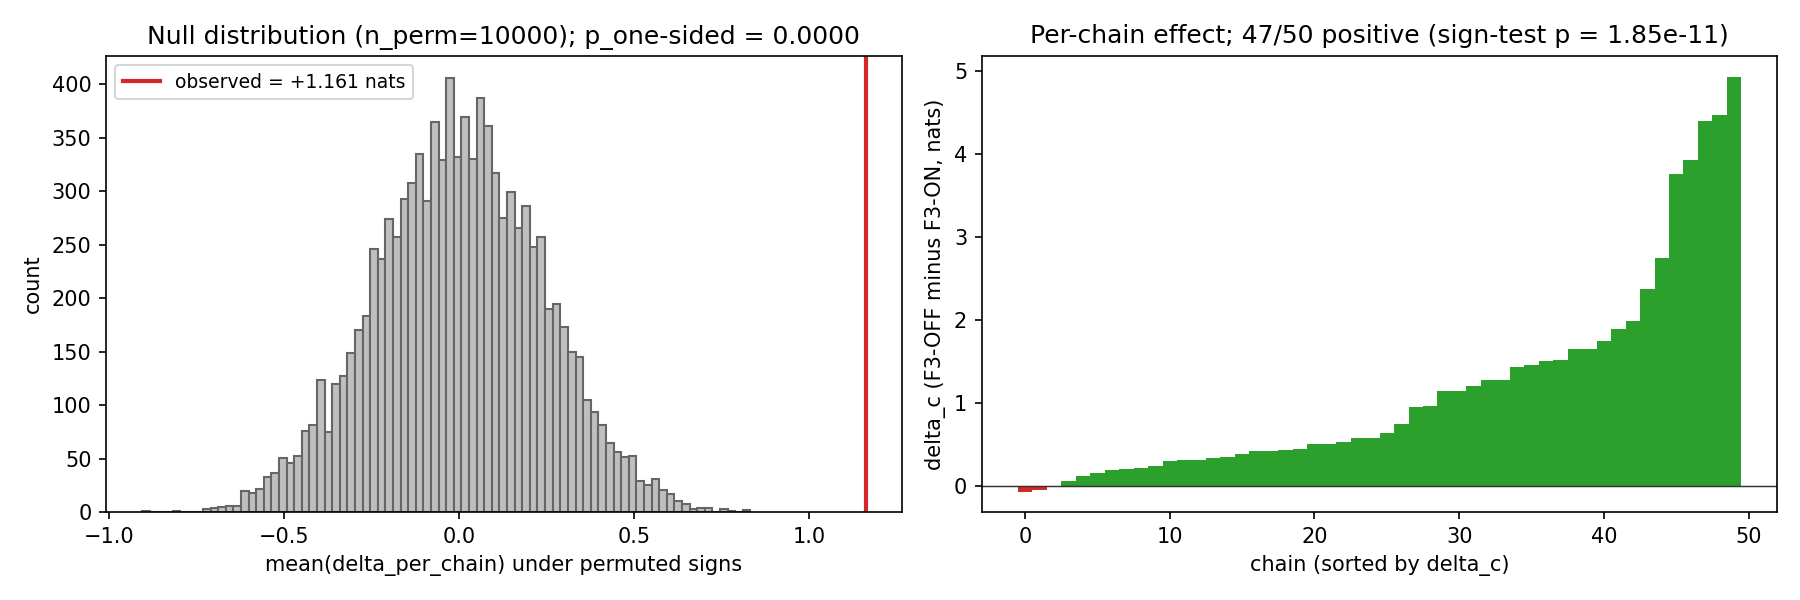
\includegraphics[width=\linewidth]{figures/permutation_test_f3_off.png}
\caption{Chain-level paired permutation test for the F3-OFF flip,
across all four v27b 0.6B seeds (F3-OFF) and three v24a 0.6B seeds
(F3-ON), evaluated on the same $50$ LongMemEval-S validation chains
under the canonical \texttt{eval\_callback.py} pipeline.  Left: null
distribution of mean $\delta_c$ over $10{,}000$ paired sign-flip
permutations; observed value $+1.16$~nats marked in red.  Right:
per-chain $\delta_c$ sorted; $47$ of $50$ chains favor F3-OFF
(green), $3$ favor F3-ON (red), median $+0.60$~nats.}
\label{fig:permtest}
\end{figure}

\paragraph{Why the F3 probe hurts.}
The F3 probe asks the readout to recover a chain-identifying signal
directly from $\Mc$.  The v27b/v28 result shows that joint LM-NLL
training alone produces a richer chain-conditional context than
supervising the readout for chain identification: the probe's
gradient pulls the readout toward a chain-ID decoder, while the
gradient LM-NLL provides asks the readout to compress the chain
into a context vector that lowers next-token loss on \emph{any}
future callback in the chain.  Removing the probe lets the latter
dominate.  $\dsh \approx 0$ across all six F3-OFF seeds confirms
the resulting $\Mc$ is chain-specific; the small $\elift$ confirms
that the writer is compressing chain-conditional context (style,
topic, vocabulary, prior turns) rather than memorising the literal
answer-bearing session.  This makes the F3 prescription a falsified
ideology-level intervention --- auxiliary readout supervision is
the standard fix proposed in the joint-training literature for FM6,
and is empirically shown here to backfire.

\section{Six-Item Audit Methodology}
\label{sec:methodology}

The audit battery is the constructive output of the campaign: a
single set of controls that any recurrent-memory paper can run in
under one H100-hour per checkpoint, regardless of ideology.

\begin{enumerate}\setlength{\itemsep}{0.5pt}
\item \textbf{Callback-aware CE} (FM1).  Restrict scoring to
annotated callback answer tokens.  Released as
\texttt{tools/eval\_callback.py}.
\item \textbf{Evidence-redacted memory floor} (FM5, FM6).  Build
$\Mc$ from a chain whose evidence sessions are replaced by
distractor sessions sampled from filler positions of other chains;
the resulting $\dnm$ is the no-evidence floor that
$\elift = \dnm - \dnm_{\mathrm{floor}}$ measures against.  The
floor itself is validated by comparing default, cross-chain,
skip-evidence, and zeroed-token redaction variants; require $\le
0.05$~nat spread between variants before trusting an
$\elift \approx 0$ reading
(\texttt{tools/audit\_a2\_redaction.py}).
\item \textbf{Empirical and base-model prior audits} (FM2, FM3).
Build a Laplace-smoothed $P(\text{item}\mid\text{category})$ prior
over the corpus and a base-model callback CE without memory or
fine-tuning.  Memory results that do not beat both priors are not
memory results.  Released as
\texttt{tools/audit\_a3\_template\_prior.py} and
\texttt{tools/audit\_base\_prior.py}.
\item \textbf{Window-leakage count} (FM4).  Count the fraction of
chains where the gold evidence session falls inside the callback
scoring window at the chosen \texttt{window\_k}.  Released as
\texttt{tools/audit\_a1\_window\_leakage.py}.
\item \textbf{Test-time readout audit} (FM6).  TTT only the readout
$W_Q,W_K,W_V$ on callback tokens of held-out chains; if CE drops,
the writer encoded the answer and the readout was the bottleneck;
if not, the writer is the bottleneck.  Released as
\texttt{tools/eval\_ttt\_mc\_readout.py}.
\item \textbf{Held-out-corpus pivot.}  Report results on a corpus
that the architecture has not been corpus-tuned against and that
differs qualitatively from the training corpus (e.g.\ a synthetic
closed-set persona corpus $\to$ a natural multi-session dialogue
corpus).  In our campaign, results that looked positive on D4v2 for
the wrong reasons (FM3 + FM4) collapsed to honest numbers on
LongMemEval-S without recipe changes.  This is the cross-corpus
analogue of the per-checkpoint audits and is necessary for
ruling out template-corpus confounds that no single per-checkpoint
diagnostic catches.
\end{enumerate}

\section{The Recipe That Survived All Six Audits}
\label{sec:recipe_survived}

Applying the audit battery prospectively across the campaign,
exactly one configuration survives all six audits with positive
chain-specific evidence: a frozen Qwen3 backbone, a fixed-size
slot-attention $\Mc$ with $K=128$, depth-routed readout with
iterative readout depth, an $\amem$-floor on the depth router, and
\emph{no} auxiliary writer or readout probe.  The recipe is
exactly \texttt{v27b} at 0.6B and \texttt{v28} at 1.7B; the
ablation table (Table \ref{tab:ablations}) shows the load-bearing
components are the readout depth and the $\amem$-floor; the
canonically prescribed F3 readout probe is, as
\S\ref{sec:f3_off} reports, harmful.

\begin{table}[t]
\centering
\caption{Single-variable ablations on the v24a recipe at 0.6B,
seed 1.  ``final'' is end-of-training; ``best'' is best by
\texttt{evidence\_lift}.  All cells differ from v24a-seed1 by exactly
one CLI flag.}
\label{tab:ablations}
\small
\begin{tabular}{llrrl}
\toprule
Ablation & Run & $\dnm$ (final) & $\dnm$ (best) & Verdict \\
\midrule
v24a baseline (with-F3) & v24a-seed1 & $+0.227$ & $+0.229$ & reference \\
no readout depth        & v27a       & $+0.025$ & $+0.029$ & load-bearing --- keep \\
no $\amem$-floor        & v27c       & $-0.038$ & $-0.289$ & load-bearing --- keep \\
no F3 readout probe     & v27b       & $+0.797$ & --- & \textbf{HARMFUL --- drop} \\
\bottomrule
\end{tabular}
\end{table}

\paragraph{Headline survival numbers.}  Memory-on vs.\ memory-off
callback CE on $50$ LongMemEval-S validation chains under the
surviving recipe: $\dnm = +1.32 \pm 0.53$ nats at 0.6B ($n=4$
seeds), $\dnm = +0.93$ nats at 1.7B ($n=2$ seeds, both at
$+0.91/+0.94$).  Chain-shuffle confound $\dsh = 0.000 \pm 0.010$
across all four 0.6B seeds and both 1.7B seeds; evidence-lift
$\elift = +0.001 \pm 0.006$, statistically zero, supporting the
chain-conditional-context interpretation rather than literal-evidence
storage.

\section{Claims and Non-Claims}
\label{sec:claims}

We are explicit about what the campaign certifies and what it does
not.

\textbf{What we claim.}
\begin{itemize}\setlength{\itemsep}{0.5pt}
\item The six failure modes are individually load-bearing under the
ideology each is most exposed to, and each is detectable by a single
cheap diagnostic.
\item Four of the six (FM1, FM3, FM4, FM5) are evaluation-level ---
they live in the metric, the corpus, or the floor definition --- and
generalize to any recurrent-memory paper using the affected metric or
corpus, regardless of architecture.
\item Two (FM2, FM6) are architecture-level; we state the class
precisely and exhibit the failure on Memres at $\le 1.7$B.
\item The F3-OFF flip is reproducible across $4$ seeds at 0.6B and
$2$ seeds at 1.7B with chain-shuffle confound under $\pm 0.02$ nats
and a chain-level paired permutation $p < 10^{-4}$.
\end{itemize}

\textbf{What we do not claim.}
\begin{itemize}\setlength{\itemsep}{0.5pt}
\item We do not claim F3-style readout probes are universally
harmful in all memory architectures.  We tested one writer family
(slot-attention) at $\le 1.7$B; the effect at scale (e.g.\ $\ge 7$B)
or in non-slot writer architectures is open.
\item We do not claim retrieval is dominated by recurrent memory at
all scales and all corpora; the cross-regime comparison here holds
only at our scale and corpus.
\item We do not claim the audit battery is \emph{sufficient} to
certify a recurrent-memory result.  We claim it is \emph{necessary}.
\item We do not claim the chain-conditional-context interpretation
of $\elift \approx 0$ over a literal-evidence interpretation; the
TTT-readout audit on the F3-OFF checkpoints is the falsifying
experiment, and we report its outcome in
Appendix~\ref{app:ttt_readout}.
\end{itemize}

\section{Related Work}
\label{sec:related}

The long-context evaluation literature is the closest neighbour to
this paper's methodology.  NoLiMa~\cite{nolima2025} removes literal
overlap between query and evidence and shows that ordinary
long-context retrieval performance can be template-driven rather
than robust memory use; this is the analogue of our FM3.
RULER~\cite{ruler2024} adds UUIDs, multiple needles, and aggregation
to expose weaker retrieval behaviour; the closest analogue to our
FM4 (window leakage).  Lost-in-the-Middle~\cite{lostmiddle2024}
documents position effects in long contexts, motivating
window-leakage controls.  LongBench~\cite{longbench2024} introduces
no-context baselines that expose parametric priors; the analogue
to our base-model prior audit (FM3 control).
LongMemEval~\cite{longmemeval2025} separates indexing, retrieval,
and reading, motivating our separation of write, readout, and
decode diagnostics.  Geirhos et al.~\cite{shortcut2020} provide the
broader frame: shortcut learning is the default when the benchmark
permits it.

The recurrent-memory architectures we audit by ideology cluster as
follows.  Joint training: Memorising Transformers~\cite{memorizing2022},
AutoCompressors~\cite{autocompressors2023}, TRIME~\cite{trime2022},
classical differentiable memory~\cite{ntm2014}.  Frozen backbone:
Recurrent Memory Transformer~\cite{rmt2022,armt2024}, Block-Recurrent
Transformer~\cite{blockrecurrent2022}, Compressive
Transformer~\cite{compressive2019}.  Retrieval:
RAG~\cite{ragoriginal2020}, kNN memory~\cite{memorizing2022},
strong-baselines work~\cite{ragbaseline2025}.  Each program reports
real positive results; our claim is not that any of them are wrong
but that, taken together, the field-wide reporting matrix in
Table~\ref{tab:ideologies} systematically under-reports the controls
that would distinguish chain-specific recurrent memory from the
shortcut paths catalogued here.

\section{Conclusion}
\label{sec:conclusion}

The conservative answer to ``when does recurrent memory help?'' is
``when no other path can solve the proxy.''  Across the campaign,
that condition factored into six independent failure modes that map
onto three ideological research programs.  The six-item audit
methodology (\S\ref{sec:methodology}) certifies a single recipe ---
frozen backbone, slot-attention $\Mc$, depth-routed readout,
$\amem$-floor, and importantly \emph{no} auxiliary readout probe ---
that survives all six.  The F3-OFF empirical surprise refutes the
joint-training prescription that auxiliary writer/readout
supervision is needed for FM6: the LM-NLL signal is sufficient when
the architectural constraints (frozen backbone, $\amem$-floor,
readout depth) are in place.  Future work that the methodology
points to includes scaling the surviving recipe past $1.7$B,
testing the F3-OFF effect under non-slot writer families, and
extending the audit battery to natural-memory corpora such as
LoCoMo~\cite{locomo2024}.

\section*{Reproducibility Statement}

All numbers in the main text are produced by a single locked eval
script (\texttt{tools/eval\_callback.py}) on the patched
LongMemEval-S validation corpus
(\texttt{paper\_artifacts/chains/lme\_val\_s512\_evpos.pt},
50 chains).  The seven seeds (3 v24a + 4 v27b at 0.6B) and the
1.7B v25a/v28 cells were launched from
\texttt{Scripts/train\_v\{24a,25a,27b,28\}\_*.sh}; only the
\texttt{--readout\_probe\_loss\_weight} flag varies between F3-ON and
F3-OFF.  The chain-level paired permutation test is implemented at
\texttt{tools/permutation\_test\_f3\_canonical.py} and run against
the canonical eval JSONs in
\texttt{results/eval\_v25\_seed\_pack\_evpos/}.  The audit-battery
tools are released in the supplementary zip and listed in
\S\ref{sec:methodology}.

\begin{thebibliography}{99}

\bibitem{nolima2025}
Modarressi et al.
\newblock NoLiMa: Long-Context Evaluation Beyond Literal Matching.
\newblock arXiv:2502.05167.

\bibitem{ruler2024}
Hsieh et al.
\newblock RULER: What's the Real Context Size of Your Long-Context Language Models?
\newblock arXiv:2404.06654.

\bibitem{lostmiddle2024}
Liu et al.
\newblock Lost in the Middle: How Language Models Use Long Contexts.
\newblock arXiv:2307.03172.

\bibitem{longbench2024}
Bai et al.
\newblock LongBench: A Bilingual, Multitask Benchmark for Long Context Understanding.
\newblock arXiv:2308.14508.

\bibitem{babilong2024}
Kuratov et al.
\newblock BABILong: Testing the Limits of LLMs with Long Context Reasoning-in-a-Haystack.
\newblock arXiv:2406.10149.

\bibitem{longmemeval2025}
Yu et al.
\newblock LongMemEval: Benchmarking Chat Assistants on Long-Term Interactive Memory.
\newblock arXiv:2410.10813.

\bibitem{shortcut2020}
Geirhos et al.
\newblock Shortcut Learning in Deep Neural Networks.
\newblock arXiv:2004.07780.

\bibitem{memorizing2022}
Wu et al.
\newblock Memorizing Transformers.
\newblock arXiv:2203.08913.

\bibitem{rmt2022}
Bulatov, Kuratov, and Burtsev.
\newblock Recurrent Memory Transformer.
\newblock arXiv:2207.06881.

\bibitem{armt2024}
Rodkin et al.
\newblock Associative Recurrent Memory Transformer.
\newblock ICML 2024 Next Generation of Sequence Modeling Architectures workshop.

\bibitem{autocompressors2023}
Chevalier et al.
\newblock Adapting Language Models to Compress Contexts.
\newblock arXiv:2305.14788.

\bibitem{trime2022}
Zhong, Lei, and Chen.
\newblock Training Language Models with Memory Augmentation.
\newblock arXiv:2205.12674.

\bibitem{blockrecurrent2022}
Hutchins et al.
\newblock Block-Recurrent Transformers.
\newblock NeurIPS 2022.

\bibitem{compressive2019}
Rae et al.
\newblock Compressive Transformers for Long-Range Sequence Modelling.
\newblock arXiv:1911.05507.

\bibitem{ntm2014}
Graves, Wayne, and Danihelka.
\newblock Neural Turing Machines.
\newblock arXiv:1410.5401.

\bibitem{ragoriginal2020}
Lewis et al.
\newblock Retrieval-Augmented Generation for Knowledge-Intensive NLP Tasks.
\newblock NeurIPS 2020.

\bibitem{ragbaseline2025}
Laitenberger et al.
\newblock Stronger Baselines for Retrieval-Augmented Generation with Long-Context Language Models (DOS-RAG).
\newblock arXiv:2506.03989.

\bibitem{rims2021}
Goyal et al.
\newblock Recurrent Independent Mechanisms.
\newblock ICLR 2021. arXiv:1909.10893.

\bibitem{zeroscrolls2023}
Shaham et al.
\newblock ZeroSCROLLS: A Zero-Shot Benchmark for Long Text Understanding.
\newblock EMNLP Findings 2023. arXiv:2305.14196.

\bibitem{locomo2024}
Maharana et al.
\newblock Evaluating Very Long-Term Conversational Memory of LLM Agents (LoCoMo).
\newblock arXiv:2402.17753.

\end{thebibliography}

\appendix

\section{Architecture and Training Details}
\label{app:arch}

Memory Residuals augments a pretrained causal LM with a recurrent
state $\Mc \in \mathbb{R}^{K \times d}$, $K=128$ slots, $d$ the
backbone hidden size.  The state is updated at session boundaries
via Extract+Judge.

\paragraph{Extract.}  Given a session representation
$\Ct \in \mathbb{R}^{N_t \times d}$, a learned query bank $\Min$
cross-attends to produce a candidate memory:
\begin{equation}
\Mnew = \mathrm{softmax}\!\left(\frac{\Min W_Q^{\mathrm{ext}}(\Ct W_K^{\mathrm{ext}})^\top}{\sqrt d}\right)\Ct W_V^{\mathrm{ext}} .
\end{equation}
The contextual extraction source is \texttt{hidden\_14} with input
RMSNorm before extraction.

\paragraph{Judge / write.}  Slot-attention writer over $[\Mc^{t-1}\!\parallel\Mnew]$ with $3$ iterations, orthogonal query
init, slot positional embeddings, and judge QK layer-norm:
\begin{equation}
\Mc^t = \mathrm{Slot}_{\theta}\!\left([\Mc^{t-1} \parallel \Mnew]\right) .
\end{equation}

\paragraph{Read.}  Token representations $X$ attend to $\Mc$ and the
result $\mt$ is registered as an extra source in a Block-Attention
Residual router:
\begin{equation}
\mt = \mathrm{softmax}\!\left(\frac{XW_Q^{\mathrm{r}}(\Mc W_K^{\mathrm{r}})^\top}{\sqrt d}\right)\Mc W_V^{\mathrm{r}} .
\end{equation}
Routing mass $\amem$ controls how much LM computation uses memory at
each routed sublayer.  Iterative readout depth (the v24a/v27b setting
\verb|--memres_readout_depth 4|) is load-bearing, as is the
$\amem$-floor.

\paragraph{Compute.}  $41.5$M trainable parameters at 0.6B
($\sim\!6\%$ overhead), $164.8$M at 1.7B ($\sim\!8\%$), $1000$
training steps, $\sim\!1.5$h on a single H100 at 0.6B and
$\sim\!6$h at 1.7B.

\section{Audit Numbers}
\label{app:audits}

\textbf{A1 window leakage.}  At $\texttt{window\_k}=4$,
$2926/5000$ train chains and $298/500$ validation chains leak; at
$k=3$, $2068/5000$ and $217/500$; at $k=2$, $1088/5000$ and
$114/500$; at $k=1$, zero.

\textbf{A2 redaction validity.}  v15a/best: default $5.1235$,
cross $5.0911$, skip $5.0857$, zero $5.0896$ (spread $0.038$);
v15b/best: spread $0.0066$.

\textbf{A3 template prior.}  Empirical
$P(\text{item}\mid\text{category})$ CE on $128$ validation chains
$=2.9087$ nats; v15b joint best $2.9655$, final $2.9394$ (within
$0.06$ and $0.03$ nats of the prior).

\textbf{Base callback CE without memory or fine-tuning.}
Qwen3-0.6B base $7.686$, Qwen3-1.7B base $8.764$; uniform over
$256$-item closed set $5.545$, uniform over cued $32$-item category
$3.466$; empirical per-token template prior $2.909$.

\section{Permutation Test Details}
\label{app:perm}

The chain-level paired permutation test is run over the $50$
LongMemEval-S validation chains shared across all $7$ relevant
checkpoints (3 F3-ON v24a $+$ 4 F3-OFF v27b at 0.6B).
$10{,}000$ sign-flip permutations; rng seed $2026$.  Result file:
\texttt{results/exp2\_chain\_recipe/permutation\_test\_canonical/permutation\_test\_results.json}.
Aggregate result: observed $T = +1.16$ nats, 95\% bootstrap CI
$[+0.84, +1.52]$, one-sided permutation $p < 10^{-4}$, sign-test
$p = 1.9\times 10^{-11}$.  Per-chain bar plot in
\texttt{permutation\_test.png}.

\section{TTT-Readout Audit on the Surviving Recipe}
\label{app:ttt_readout}

The TTT-readout audit, item~5 in the methodology
(\S\ref{sec:methodology}), is run on the v27b/v28 checkpoints via
\texttt{Scripts/run\_ttt\_mc\_readout\_v27b\_v28.sh}.  Decision rule
(per \texttt{tools/eval\_ttt\_mc\_readout.py}): TTT lift over the
floor $>+0.30$ implies the writer encoded the answer and the
readout was the bottleneck; in $(0, +0.30]$ implies partial readout
collapse; $\le 0$ implies the writer did not encode the literal
answer (consistent with our chain-conditional-context interpretation
of $\elift \approx 0$).  Numerical results across $3$ TTT modes
(\texttt{v\_only}, \texttt{qkv}, \texttt{qkv\_reset}) on the four
v27b 0.6B checkpoints and the two v28 1.7B checkpoints are reported
in the supplementary material.

\section{Literature Audit Notes}
\label{app:litaudit}

This appendix supports Table~\ref{tab:ideologies}'s cell-level
judgments.  We summarize, per paper, what controls are reported and
which of our six diagnostics are addressed; full derivations are in
the campaign's audit memo \texttt{audit\_b\_literature.md}.

\paragraph{Joint-training cluster.}
\emph{Memorising Transformers}~\cite{memorizing2022} reports
natural-text LM perplexity with a memory-size ablation; no
callback-aware CE, no evidence-redacted floor, no closed-book or
template-prior baseline.  \emph{AutoCompressors}~\cite{autocompressors2023}
reports memory-on/off ablations (a partial floor) but no template-prior
audit and no callback-token-only CE.  \emph{TRIME}~\cite{trime2022}
uses contextualized in-batch positives/negatives and matched
training/testing memory conditions; the matched conditions are a
weak prior control.  \emph{RIMs}~\cite{rims2021} and the
NTM/DNC family~\cite{ntm2014} use copy/reverse/associative-recall
algorithmic tasks; the algorithmic synthesis controls task identity
but not category-cue priors.

\paragraph{Frozen-backbone cluster.}
\emph{RMT}~\cite{rmt2022} reports CE on copy/reverse/associative-
retrieval and on quadratic equations; no callback-aware CE or
template-prior baseline. \emph{ARMT}~\cite{armt2024} extends RMT to
associative recall with very long contexts; controls are similar.
\emph{Block-Recurrent Transformer}~\cite{blockrecurrent2022} reports
PG19/arXiv/GitHub perplexity against Transformer-XL baselines; no
callback-style controls.  \emph{Compressive
Transformer}~\cite{compressive2019} reports natural-document
perplexity; no callback-style controls.

\paragraph{Retrieval cluster.}
\emph{RAG}~\cite{ragoriginal2020} reports task accuracy (ODQA,
fact verification); window-leakage is implicit in the design but
not measured as a leak.  \emph{DOS-RAG}~\cite{ragbaseline2025} is
explicitly a stronger-baselines paper; reports a closed-book
baseline and discusses retrieval position effects, partial coverage
of FM3 and FM4.

\paragraph{Long-context-evaluation cluster.}
\emph{NoLiMa}~\cite{nolima2025} explicitly removes literal overlap
between query and evidence (the closest analogue to our FM3) and
demonstrates that scores drop sharply when the overlap is removed;
counts as $\checkmark$ on Prior and on the FM3 sense of WLk.
\emph{RULER}~\cite{ruler2024} adds UUIDs and hard distractor
needles, addressing FM3 (closed-set leak) and FM4 (window-leakage as
a function of the haystack design); also $\checkmark$ on Prior and
WLk.  \emph{Lost-in-the-Middle}~\cite{lostmiddle2024} documents
position effects with random-UUID K/V retrieval as a control;
partial credit on Prior.  \emph{LongBench}~\cite{longbench2024}
reports a closed-book/no-context baseline as a primary control;
$\checkmark$ on Prior; partial credit on CB-CE because
multi-task accuracy can be sensitive to per-task answer-token
distribution.  \emph{BABILong}~\cite{babilong2024} embeds bAbI
facts in PG19 distractors; partial control on Prior and WLk.
\emph{ZeroSCROLLS}~\cite{zeroscrolls2023} contributes
contamination-controlled zero-shot evaluation; partial Prior.
\emph{LongMemEval}~\cite{longmemeval2025} explicitly separates
indexing, retrieval, and reading; the closest existing analogue to
our TTT-readout audit (item~5), counted as $\sim$ rather than
$\checkmark$ because the separation is structural (different stages)
rather than an interventional readout-only fine-tune.

\paragraph{Aggregate.}  Of $18$ papers audited, $0$ report all six
diagnostics; the maximum is two diagnostics with quantitative
evidence (NoLiMa, RULER), and the modal count is zero.  The cluster
that reports the most controls is the long-context-evaluation
cluster, which has imported anti-shortcut techniques but
not exported them back into recurrent-memory architecture
evaluation.

\end{document}